%! suppress = NonBreakingSpace
\documentclass[a4paper,12pt]{article}
\usepackage[finnish]{babel}
\usepackage{layout}
\usepackage{graphicx}
\usepackage{geometry}
\usepackage{blindtext}
\usepackage{lastpage}
\usepackage{listings}
\usepackage{multirow}
\usepackage{amsmath}
\usepackage{url}
\usepackage{listings}
\usepackage{listings-rust}
\usepackage{tikz}
% \usepackage{showframe}
\lstset{language=Rust, style=boxed,
 literate={ö}{{\"o}}1
           {ä}{{\"a}}1
}
\renewcommand{\lstlistingname}{Lähdekoodi}

\usepackage{tikz}
\usetikzlibrary{positioning,shapes,shadows,arrows}

\tikzstyle{struct}=[rectangle, draw=black, text centered, anchor=north, text=black, text width=4cm]
\tikzstyle{thread}=[rectangle, draw=black, text centered, anchor=north, text=black, text width=4cm]
\tikzstyle{app}=[rectangle, draw=black, text centered, anchor=north, text=black, text width=3cm]



\newcommand{\architecture}{
\begin{figure}[h!]
\centering
    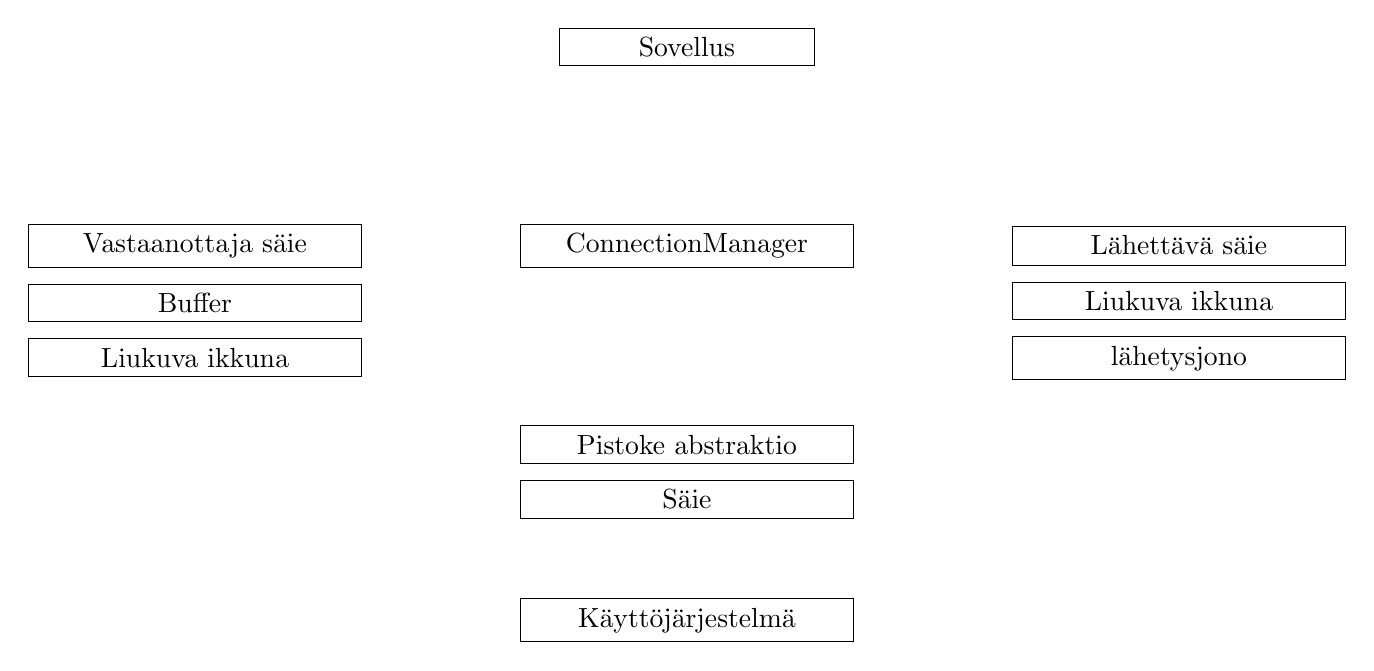
\begin{tikzpicture}[node distance=2cm]
        \node(app)[app]{
            Sovellus
        };
        \node(ConnectionManager)[struct, below=of app] {
            ConnectionManager
        };
       \node(rthread)[thread, left=of ConnectionManager]{
            Vastaanottaja säie
       };
       \node(buffer)[struct, below=0.2cm of rthread] {
            Buffer 
       };
       \node(rwindow)[struct, below=0.2cm of buffer] {
            Liukuva ikkuna 
       };
       \node(tthread)[thread, right=of ConnectionManager]{
            Lähettävä säie
       };
       \node(twindow)[struct, below=0.2cm of tthread] {
            Liukuva ikkuna 
       };
       \node(queue)[struct, below=0.2cm of twindow] {
            lähetysjono
       };
       \node(socket)[struct, below=of ConnectionManager]{
            Pistoke abstraktio
       };
       \node(socketthread)[struct, below=0.2cm of socket]{
            Säie
       };
       \node(os)[struct, below=1cm of socketthread]{
            Käyttöjärjestelmä
       };
    \end{tikzpicture}
    \caption{Arkkitehtuuridiagrammi} \label{fig:arkkitehtuuri}
\end{figure}
}








\title{Luotettava UDP-yhteys}
\author{Joonas Kajava}
\date{\today}

\newcommand{\me}{Joonas Kajava}
\renewcommand{\title}{Luotettava UDP-yhteys}

\newcommand{\appendixCount}{0}

\newcommand{\pageCount}{ \pageref{LastPage}}

\newcommand*\sepline{
    \begin{center}
        \rule[1ex]{\textwidth}{.5pt}
    \end{center}}


\begin{document}
    \begin{titlepage}
        
\includegraphics[width=0.5\textwidth]{images/metropolia}\par\vspace{2cm}
        {\Large \me}\par \vspace{1cm}

        {\Huge \title}\par \vspace{1cm}

        \vfill

        Metropolia Ammattikorkeakoulu\par
        Insinööri (AMK)\par
        Tieto ja viestintätekniikka\par
        Insinöörityö\par
        \today

        \newpage
        \thispagestyle{empty}

        \section*{Tiivistelmä}

        \begin{tabular} {l l}
            Tekijä:               & \me                                            \\
            Otsikko:              & \title                                         \\
            Sivumäärä:            & \pageCount{} sivua + \appendixCount{} liitettä \\
            Aika:                 & \today                                         \\
            \\
            Tutkinto: & Insinööri (AMK) \\
            Tutkinto-ohjelma: & Tieto- ja viestintätekniikka \\
            Ammatillinen pääaine: & Ammatillinen pääaine \\
            Ohjaajat: & Tehtävänimike Etunimi Sukunimi                      \\
            & Tehtävänimike Etunimi Sukunimi \\
        \end{tabular}
        \sepline
        \newpage
        \thispagestyle{empty}


        \tableofcontents
        \newpage
        \thispagestyle{empty}


        \section*{Lyhenteet}
        \begin{tabular}{l l}
            UDP: & User Datagram Protocol        \\
            TCP: & Transmission Control Protocol \\
            IP:  & Internet Protocol             \\
            ACK: & Acknowledgement               \\
            NAK: & Negative Acknowledgement      \\
            NIC: & Network Interface Controller  \\
        \end{tabular}
        \newpage


    \end{titlepage}


    \section{Johdanto}\label{sec:johdanto}
    Tässä työssä käsitellään teoria internet protokollan luomiseen. Teorian jälkeen lukija ohjataan vaiheittan internet protokollan luomiseen UDP:n päälle. Tämän työn tarkoitus on luoda pohja yrityksille ja kehittäjille, minkälainen on internet protokollan toteutus ja mihin asioihin täytyy ottaa huomiota.
    \par Työ on luonteeltaan tutkivaa ja tarkoitus on luoda selkeä pohja minkä perusteella on yksinkertaista hyödyntää UDP-protokollaa reaaliaikaisiin ohjelmiin.


    \section{Internet-protokollat}
    TCP ja UDP protokollat ovat kaksi yleisintä TCP/IP protokollaa.
    Näistä TCP protokolla on usein käytetty palveluissa, jotka vaativat vakaata ja luotettavaa yhteyttä. UDP paras reaaliaikaisia sovelluksia varten. Tämä johtuu siitä, että TCP paketin mukana liikkuu paljon reservoituja tavuja, joita ei käytetä ollenkaan, myös otsikko päättyy turhaan täytteeseen.
    \par
    UDP:n etu realiaikaisessa kommunikaatiossa on, että se on kevyt ja nopea.
    \cite{KumarSurveyUDP}
    \par



    \section{Tavoitteet ja motivaatio}
    Tämän työn tavoitteena on internet protokollien toimintaa ja niiden implementointia. Tilanteissa missä kaistanleveys on rajallinen ja nopea vasteaika on tärkeää, on usein kannattavaa luoda oma protokolla, joka on räätälöity sovelluksen tarpeita varten.
Oman protokollan käyttöönotto vaatii kohtuullisen määrän tietoa verkkosovittimien, UDP protokollan, yhtäaikaisuudesta sekä tehokkaista tietorakenteista.\par
    Tässä dokumentissa käydään läpi internet protokollien teoriaa, toteutukset käyttäen rust ohjelmointi kieltä ja lopuksi tutkiva osuus jossa mitataan protokollien suorituskykyä ja tehokkuutta.


    \section{Verkkosovitin}\label{sec:verkkosovitin}
    Rust-ohjelmointikieli käyttää linuxissa \textit{libc}-kirjastoa \cite{rust-source-unix-netrs}

    \section{Verkkopistoke}\label{sec:verkkopistoke}
    \blindtext


    \section{TCP/IP}\label{sec:tcpip}
    \blindtext

    \section{Paketti}\label{sec:paketti}
    Paketti on perustuu TCP:n ja on rakennettu UDP:n päälle. Paketin rakenne on minimaalinen ja yksinkertainen.

\begin{align}
    \text{Frame size} &= F_s \\
    \text{Option size} &= O_s = F_s - F_{min} - D_s
\end{align}



\begin{table}[h!]\
    \centering
    \resizebox{\textwidth}{!}{
        \begin{tabular}{*{33}{|l}|l|}
        \hline
        \multicolumn{2}{|c|}{Offsets} & \multicolumn{8}{|l|}{0}& \multicolumn{8}{|l|}{1}& \multicolumn{8}{|l|}{2}& \multicolumn{8}{|l|}{3} \\ \hline
        Octet & Bit&0&1&2&3&4&5&6&7&0&1&2&3&4&5&6&7&0&1&2&3&4&5&6&7&0&1&2&3&4&5&6&7 \\ \hline
        0 & 0 & \multicolumn{32}{|c|}{Sequence number} \\ \hline
        4&32&RES&RES&RES&RES&RES&RES&EOM&ACK&\multicolumn{8}{|c|}{Reserved}&\multicolumn{8}{|c|}{Data Length}&\multicolumn{8}{|c|}{Data Offset} \\ \hline
        32&64&\multicolumn{32}{|c|}{Options} \\
        ...&...& \multicolumn{32}{|c|}{} \\ \hline
        \multicolumn{2}{|c|}{Data Offset}&\multicolumn{32}{|c|}{Data} \\
        ...&...& \multicolumn{32}{|c|}{} \\ \hline
        \end{tabular}
    }
    \caption{Paketin rakenne}
    \label{tab:my_label}
\end{table}

Tässä työssä paketti on määritelty seuraavasti:
\begin{lstlisting}[caption={Paketin rakenne}, label={lst:frame}]
pub struct Frame {
    frame: [u8; MAX_FRAME_SIZE],
    data_length: usize,
    options_size: usize,
}
\end{lstlisting}
Lähdekoodissa \ref{lst:frame} määritetaan tietorakenne \textit{Frame},
\lstinline{[u8; MAX_FRAME_SIZE]} on taulokkotyyppi joka koostuu tavuista ja on kooltaan yhtä suuri kuin $F_{max}$.
\lstinline{data_length} sisältää tiedon pakettiin tallennetun datan koosta. \lstinline{options_size} sisältää tiedon paketin asetuksien koosta.\par
\lstinline{usize} vastaa kohde arkkitehtuurin muistiosoitteen kokoa. 32 bittisessä kohde tietokoneessa \lstinline{usize} vastaa 4 tavua ja 64 bittisessä kohteessa 8 tavua \cite{rust-doc-usize}.

\subsection{Tietojen käsittely paketissa}
    Paketti on ohjelmanmuistissa yhtenä kokonaisena taulukkona, joka koostuu tavuista.
    Paketti sisältää tietoja 16 bittisessä ja 32 bittisessä muodossa. Nämä tiedot täytyy jakaa tavuihin lähettämistä varten.

\begin{lstlisting}[caption={Järjestusnumeron asettaminen pakettiin}, label={lst:set_seq_num}]
pub fn set_sequence_number(&mut self, sequence_number: u32) {
    let net_sequence_number = sequence_number.to_be_bytes();
    self.frame[SEQUENCE_NUMBER_OCTET..4].copy_from_slice(&net_sequence_number);
}
\end{lstlisting}

Lähdekoodissa \ref{lst:set_seq_num} järjestysnumero muutetaan laskevaan tavujärjestykseen, käyttäen rust standardi kirjaston functiota \lstinline{to_be_bytes()} \cite{rust_doc_u32}. Tämän jälkeen se kopiodaan paketin 4 ensimmäisen tavun tilalle. \par
Oikea tavujärjestys on erittäin tärkeä osa tiedon siirrossa verkon ylitse. Protokollaa käyttävät tietokoneet täytyvät olla yhteisymmärryksessä mitä tavujärjestystä tiedonsiirrossa käytetään. laskeva tavujärjestys on yleisn järjestys, joten päätin käyttää sitä myös tässä protokollassa. \par
Mikäli tavujärjestystä ei ota huomioon tiedonsiirrossa ja vastaanottaja sekä lähettäjän tietokoneet käyttävät eriävää tavujärjestystä, lukujen muuntaminen tavutaulukosta primitiiviseksi luvuksi tuottaa vääriä tuloksia.
\cite{Adiga2007HowC}
// TODO: Lisää jotain diagrameja tähän

    \subsection{Kuljetuskerros}\label{subsec:kuljetuskerros}
    Kuljetuskerros hoitaa pakettien luomisen ja välittämisen paketin verkkosovittimeen.
    Kuljetuskerros määrittelee seuraavat osat protokollasta:

    \begin{itemize}
        \item Paketteihin liittyvät vakiot
        \item Ohjausbitit
        \item Paketin otsakkeen
        \item Paketin lisäasetukset
        \item Vastaanottoikkunan toiminnan
        \item Lähetysikkunan toiminnan
    \end{itemize}

    \subsection{Vakiot}
    Vakiot ovat tärkeitä protokollan toiminnan kannalta. Vastaanottajalla ja lähettäjällä täytyy olla samat vakiot käytössä jotta pakettien muodostaminen sekä lukeminen onnistuu.


    \begin{table}[h!]
        \centering
        \begin{tabular}{llll}
            Vakion-nimi & Lyhenne & Arvo & Yksikkö \\
            \hline
            MAX\_DATA\_SIZE & $D_s$ & 128 & Tavu \\
            SEQ\_NUM\_SIZE & $S_s$ & 4 & Tavu \\
            CONTROL\_BITS\_SIZE & $C_s$ & 1 & Tavu \\
            RESERVED\_SIZE & $R_s$ & 1 & Tavu \\
            DATA\_LENGTH\_SIZE & $DL_s$ & 1 & Tavu \\
            DATA\_OFFSET\_SIZE & $DO_s$ & 1 & Tavu \\
            OPTION\_KIND\_SIZE & $OK_s$ & 1 & Tavu \\
            OPTION\_LENGTH\_SIZE & $OL_s$ & 1 & Tavu \\
            OPTION\_DATA\_SIZE & $OD_s$ & 4 & Tavu \\
            MAX\_OPTION\_COUNT & $MO_c$ & 4 & Määrä
        \end{tabular}
        \caption{Vakiot ja niiden arvot}
        \label{tab:vakiot}
    \end{table}

    Näiden vakioiden perusteella voidaan laskea tärkeitä muuntujia\footnote{Ohjelman kääntäjä laskee nämä ja tallentaa tulokset vakioarvoiksi \cite{rust_book_constant_evaluation}.}.

    \begin{align}
        \text{MIN\_FRAME\_SIZE} &= F_{min} = S_s + C_s + R_s + DL_s + DO_s \\
        \text{MAX\_FRAME\_SIZE} &= F_{max} = F_{min} + MO_c(OK_s + OL_s + OD_s) + D_s \label{eq:fmax}
    \end{align}


    \subsection{Ohjausbitit}
    Ohjausbitit ilmaantuvat paketissa yhtenä tavuna, joista jokainen bitti vastaa tiettyä ohjausbittiä.

    \begin{table}[h!]
        \centering
        \begin{tabular}{lll}
            Nimi & Lyhenne & Binääriarvo \\
            \hline
            Kuittaus & ACK & 00000001 \\
            Pääte & EOM & 00000010 \\
        \end{tabular}
        \caption{Ohjausbitit ja niiden arvot}
        \label{tab:control_bits}
    \end{table}

    Taulukon \ref{tab:control_bits} määrittämät ohjausbitit antavat vastaanottajalle tärkeää tietoa paketista. Kuittaus bitti ilmoittaa lähettäjälle, että vastaanottaja on saanut paketin onnistuneesti. Pääte bitti ilmoittaa vastaanottajalle, että kyseinen paketti on paketti ryhmän viimeinen ja ryhmä on valmis koottavaksi kun kaikki sitä edeltävät paketit ovat saapuneet. \par
    Vastaanottaja tarkistaa ohjausbittien olemassaolon bittioperaatiolla.
\begin{lstlisting}[caption={Kuittasbitin tarkistus ohjausbiteistä}, label={lst:ack_check}]
if control_bits & 00000001 == 00000001 {
    // Kuittaus bitti löytyy
}
\end{lstlisting}




    \subsection{Sovelluskerros}\label{subsec:sovelluskerros}
    \blindtext


    \section{UDP}\label{sec:udp}
    \blindtext


    \section{Arkkitehtuuri}\label{sec:arkkitehtuuri} 
    \architecture

     \lstinline{ConnectionManager} on vastuussa yhteyksien hallinnasta. Sen tehtävä on 
    hoitaa vastaanottaja säiettä ja lähettävää säiettä. Kun sovellus haluaa käynnistää yhteyden, 
    \lstinline{ConnectionManager} luo pistokkeen sovelluksen antamaan osoitteeseen. 
    Lähetys ja vastaanotto säikeet käynnistyvät kun pistokkeen luonti onnistuu. 
    \par
    \begin{lstlisting}[caption={ConnectionManager rakenne}, label={lst:connectionmanager}]
pub struct ConnectionManager {
    listener_thread: Option<thread::JoinHandle<()>>,
    transmitter_thread: Option<thread::JoinHandle<()>>,
    socket: Arc<SocketAbstraction>,
    message_sender: SyncSender<Vec<u8>>,
}\end{lstlisting}

\begin{lstlisting}[caption={Drop ominaisuuden toteutus ConnectionManager:ille}, label={lst:connectionmanager_drop}]
impl Drop for ConnectionManager {
    fn drop(&mut self) {
        if let Some(x) = self.listener_thread.take() {
            x.join().unwrap();
        }
        if let Some(x) = self.transmitter_thread.take() {
            x.join().unwrap();
        }
    }
}
\end{lstlisting}


    \lstinline{ConnectionManager} pitää muistissa viitteet vastaanottaja ja lähettäjä säikeisiin.
    \lstinline{Option<...>} määrittelee valinnaisen arvon, joka tarkoittaa, että kyseinen muuntuja ei 
    välttämättä sisällä käyttökelpoista arvoa. Tämä vastaa muissa useissa ohjelmointikielissä \lstinline{null} arvoa \cite{rust_book_enum}. Näitä kahta muuntujaa käytetään säikeiden sulavaan sulkemiseen kun \lstinline{ConnectionManager} pudotetaan muistista. 

    \lstinline{ConnectionManager} implementoi \lstinline{Drop} ominaisuuden, joka liittää vastaanottaja
    ja lähettäjä säikeet. Näin ohjelma jää odottamaan, että nämä kaksi säiettä sulkeuduu oikein \cite{rust_doc_joinhandle}.
        
    \section{Liukuva ikkuna}\label{sec:liukuva_ikkuna}
    \begin{lstlisting}[caption={Ikkunan rakenne}, label={lst:window}]
pub struct Window {
    frame_status: Vec<bool>,
    window_size: u32,
    window_left_edge: u32,
}\end{lstlisting}


    \begin{lstlisting}[caption={Vastaanottajan ikkunan rakenne}, label={lst:rwindow}]
pub struct ReceiverWindow {
    inner_window: Window,
    buffer: Vec<Option<Frame>>,
}\end{lstlisting}

    \begin{lstlisting}[caption={Lähettävän ikkunan rakenne}, label={lst:twindow}]
pub struct TransmitterWindow {
    inner_window: Window,
    socket: Arc<SocketAbstraction>,
    events_sender: Sender<ConnectionEventType>,
    ack_receiver: Receiver<u32>,
    data_queue: Vec<Option<QueueFrame>>,
}\end{lstlisting}

    \subsection{Ikkunan siirto vastaanottaessa}

    \begin{align}
        n_s &= \text{Pienin vastaanotettu järjestysnumero} \\
        n_x &= \text{Vastaanotetun paketin järjestysnumero} \\
        w_s &= \text{Ikkunan koko}
    \end{align}



Vastaanottajan ikkuna määritellään lähdekoodin \ref{lst:rwindow} mukaisesti. Se sisältää yleisen \lstinline{Window} toteutuksen ja \lstinline{buffer} kentän, jonka tarkoitus on pitää tietoja 
tallessa ennenkuin ne kasataan yhdeksi kokonaisuudeksi. \par
Rust-kielessä ei pysty tekemään perintää samantyylisesti kuin yleisissä OOP-kielissä. Tämän takia
käytetään suunnittelutapaa nimeltä "\textit{Composition over Inheritance}" \cite{Ivicevic202228Inheritance}.



    Vastaanottava ikkuna pitää muistissa pienimmän järjestysnumeron $n_s$, minkä se on vastaanottanut.
Vastaanottava ikkuna hylkää kaikki paketit, joiden järjestysnumero on ikkunan ulkopuolella $n_x < n_s$ tai $n_x > n_s + w_s$. Jos järjestysnumero on ikkunan sisällä, se hyväksytään ja merkitään vastaanotetuksi. Mikäli $n_x = n_s + 1$ ikkunaa voidaan siirtää eteenpäin.
    Ikkunan siirto tapahtuu kulkemalla hyväksyttyjen järjestysnumeroiden listaa eteenpäin, kunnes vastaan tulee järjestysnumero jota ei ole vielä vastaanotettu. Kulkiessa tapahtuneiden askelien määrä lisätään muuntujaan $n_s$.

    \subsection{Valikoiva toisto}\label{subsec:valikoiva_toisto}
    \blindtext

    \subsection{Kuittaus}\label{subsec:kuittaus}
    \blindtext


    \section{Virheenkorjaus}\label{sec:virheenkorjaus}
    \blindtext


    \section{Suorityskyky}
    Suorituskyvyn mittaaminen toteutetaan sisäverkossa, jotta tiedonsiirto nopeus on deterministinen ja vakaa.
    Testiympäristö koostuu yhdestä Windows tietokoneesta, joka muodostaa yhteyden itseensä käyttäen silmukka osoitetta.\par
    Testissä tietokone siirtää itselleen silmukan kautta 50 megatavun tiedoston. Testi suoritetaan 10 putkeen jotta saadaan leville keskiarvo selville.

    \subsection{Asynkroninen }
    \bibliographystyle{vancouver}
    \bibliography{doc/latex/src/mendeley}


\end{document}